
\documentclass{article}
\usepackage[utf8]{inputenc}
\usepackage[T5]{fontenc}
\usepackage{graphicx}
\usepackage[margin=1.5cm]{geometry}
\title{Lab 3: Hello, CUDA!}
\author{Nguyễn Thanh Hùng -- 2540056}
\date{}
\begin{document}
\maketitle
Each CPU iteration and each GPU thread computes $Y=0.299R+0.587G+0.114B$.
The RGB image is flattened to $(HW,3)$ for the 1D kernel. Blocks of 32--512 threads are compared.
The notebook shows both images, checks the maximum pixel error, and plots block size versus GPU time.
Select the fastest measured block; larger blocks do not necessarily run faster.

Kernel timing uses \texttt{time.time()} after JIT warm-up and CUDA synchronization,
averaged over three GPU runs. Device allocation and host/device copies are excluded.
CPU measurements are single runs. Speedup is relative to the stated CPU implementation.
Actual measurements appear after running the notebook on Colab; no timings are assumed here.
\IfFileExists{results.tex}{\begin{center}
\resizebox{\linewidth}{!}{
\begin{tabular}{lllll}
\hline
block & cpu\_ms & gpu\_ms & speedup & max\_error \\
\hline
32 & 421.821 & 0.0771681 & 5466.26 & 1 \\
64 & 421.821 & 0.0480016 & 8787.65 & 1 \\
128 & 421.821 & 0.0410875 & 10266.4 & 1 \\
256 & 421.821 & 0.0766913 & 5500.25 & 1 \\
512 & 421.821 & 0.042518 & 9921.01 & 1 \\
\hline
\end{tabular}
}
\end{center}}{}
\IfFileExists{performance.png}{\begin{center}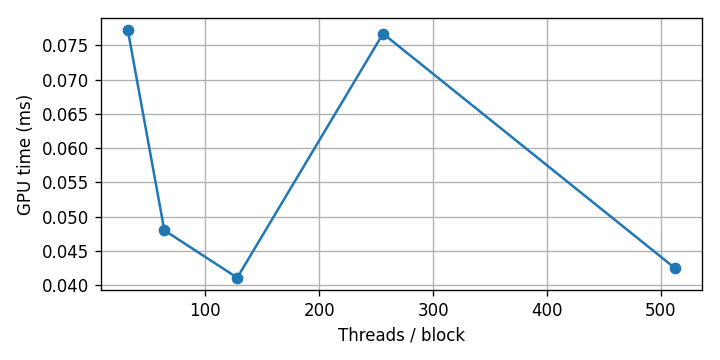
\includegraphics[width=.75\linewidth]{performance.png}\end{center}}{}
\IfFileExists{images.png}{\begin{center}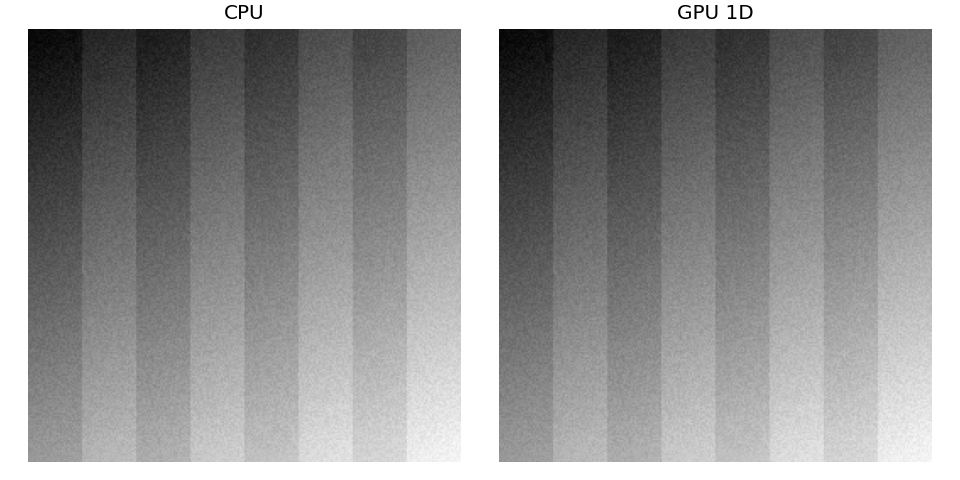
\includegraphics[width=\linewidth]{images.png}\end{center}}{}
\IfFileExists{histograms.png}{\begin{center}\includegraphics[width=.8\linewidth]{histograms.png}\end{center}}{}
\end{document}
